\documentclass[conference]{IEEEtran}
\IEEEoverridecommandlockouts
% The preceding line is only needed to identify funding in the first footnote. If that is unneeded, please comment it out.
\usepackage[utf8]{inputenc}
\usepackage{amsmath, amssymb, amsfonts}
\usepackage{algorithmic, float, graphicx, textcomp, color, xcolor, colortbl}
\usepackage{cite, hyperref, listings, pdfpages, comment, fancyhdr, subcaption, tikz}
\usepackage[margin=0.8in]{geometry}
\usepackage[english]{babel}
\usepackage{enumerate}% http://ctan.org/pkg/enumerate
\usepackage[linesnumbered,ruled,vlined]{algorithm2e}

% light gray color
\definecolor{lightgray}{gray}{0.7}

\def\BibTeX{{\rm B\kern-.05em{\sc i\kern-.025em b}\kern-.08em
    T\kern-.1667em\lower.7ex\hbox{E}\kern-.125emX}}
\begin{document}

\title{Pashto Poetry Attribution using Deep Learning Techniques}
% \title{Pashto Poetry Classification through Deep Neural Architectures}

\author{
\IEEEauthorblockN{Ali Muhammad Asad}
\IEEEauthorblockA{\textit{Computer Science} \\
\textit{Habib University}\\
Karachi, Pakistan \\
aa07190@st.habib.edu.pk}
\and
\IEEEauthorblockN{Shayan Shoaib Patel}
\IEEEauthorblockA{\textit{Computer Science} \\
\textit{Habib University}\\
Karachi, Pakistan\\
sp07101@st.habib.edu.pk}
\and
\IEEEauthorblockN{Sadiqah Mushtaq}
\IEEEauthorblockA{\textit{Computer Engineering} \\
\textit{Habib University}\\
Karachi, Pakistan \\
sm07152@st.habib.edu.pk}
\and
\IEEEauthorblockN{Lyeba Abid}
\IEEEauthorblockA{\textit{Computer Engineering} \\
\textit{Habib University}\\
Karachi, Pakistan \\
la07309@st.habib.edu.pk}
\and
\IEEEauthorblockN{Dr. Abdul Samad}
\IEEEauthorblockA{\textit{Associate Professor, CS} \\
\textit{Habib University}\\
Karachi, Pakistan \\
abdul.samad@sse.habib.edu.pk}
\and
\IEEEauthorblockN{Sandesh Kumar}
\IEEEauthorblockA{\textit{Computer Science} \\
\textit{Habib University}\\
Karachi, Pakistan \\
sandesh.kumar@sse.habib.edu.pk}
}

\maketitle
\pagenumbering{arabic}

% \begin{abstract}

%     % This paper explores the application of deep learning to the classification of Pashto poetry, aiming to preserve its literary heritage and enhance global appreciation. By leveraging neural networks, the study categorizes Pashto poems based on thematic and structural features, offering insights into its poetic forms. This classification facilitates deeper linguistic analysis and educational engagement, while also advancing machine translation and natural language processing (NLP) for Pashto, a low-resource language. Additionally, the research contributes to digital humanities by enabling large-scale analysis, fostering a bridge between technology and cultural studies.
    
% \end{abstract}



\section{Introduction}

Poetry has been a cornerstone of cultural and literary heritage across the globe, as it is one of the most popular ways to express emotions, thoughts, and experiences. Pashto is one of the major languages spoken in Afghanistan and Pakistan, with 50\% of the Afghan population speaking Pashto, and 15\% of the Pakistani population speaking Pashto \cite{ciawordlfactbook} \cite{pbs}. As such, it also holds a significant place in the rich tapestry of South Asian literature with its first recorded poetic works believed to be dating back to the 8th century with the works of Amir Kror Suri (a warrior poet) \cite{history_pashto}. There have also been other notable poets such as Khushal Khan Khattak, Rahman Baba, Ghani Khan, and Hamza Baba who have contributed to the Pashto literary tradition, and are revered for their works. However, despite its rich history and cultural significance, Pashto remains a low-resource language in the context of computational linguistics, with limited availability of annotated data and tools for natural language processing (NLP) apart from translated works. This gap poses challenges for preserving and promoting Pashto literature on a global scale. Thus, the attribution of poetic works to specific poets can sometimes be ambiguous, due to oral traditions, and lack of proper documentation. 

In recent years, deep learning techniques have gained substantial traction in the field of language processing, text classification, and poet attribution. Poet attribution refers to the process of identifying the poet who authored a specific poem. This process is crucial for preserving the cultural heritage of a language, as well as for academic research and literary studies. While researchers have explored poetry attribution in various languages such as English, Hindi, Urdu, Arabic, Persian, and Gujrati, Pashto poetry has not been extensively studied in this context. This gap could also be attributed to the lack of resources, and documentation in Pashto. This paper aims to bridge this gap by introducing deep learning based approaches to classify Pashto poetry and attribute it to specific poets, which can also prevent misinformation and mis-attribution due to the lack of proper documentation available. This paper also aims to curate the first Pashto poetry dataset of 23 poets (old and relatively newer poets) with 27,607 couplets in total, which will be made publicly available to the research community.

\section{Related Work}

Poet attribution using deep learning and machine learning has been explored in various languages previously as well. 

A recent study on the poet attribution for Punjabi poetry \cite{fatimarazapunjabipoetry} used deep learning, including transformer-based techniques for three different scripts of punjabi poetry; Gurmukhi, Shahmukhi, and Roman scripts. They curate a dataset from scratch, consisting of 830 poems from 11 punjabi poets. Their methodology includes splitting the data into 80-10-10 for training, validation, and testing, respectively, followed by tokenization and embedding generation which is then passed onto the deep learning and transformer models. They also experiment with TF-IDF vectorization instead of embeddings for the models. The trained Bi-LSTM, Bi-GRU, DistilBERT, Softmax regression, SVM, and Random Forest. The DistilBERT gave the highest accuracy for the Gurmukhi and Shahmukhi script of 90.36\% and 87.95\% respectively. The Bi-Gru follows with an accuracy of 89.16\% on the Gurmukhi script, while Bi-LSTM have the second highest accuracy of 81.93\% on the Shahmukhi script. Bi-LSTM performed the best on the roman script with an accuracy of 91.57\%, followed by SVM with an 89.16\% accuracy, and then DistilBERT with an accuracy of 87.95\%. 

A study on poet attribution for Urdu Ghazals \cite{fizza_iqra_urdu_attribution} employed machine learning, deep learning, and transformer-based techniques on a dataset of 18,609 couplets from 15 notable Urdu poets, covering both the 18th-19th and 19th-20th centuries. The distinct word usage and styles across these periods benefited the model in identifying patterns. The study tested four machine learning models — Logistic Regression, Random Forest, Naive Bayes, and SVM — using label encodings and TF-IDF for feature extraction. They also experimented with four deep learning models: Flatten, LSTM, GRU, and 1D-CNN, utilizing one-hot encoding and tokenization with a 300-dimensional embedding layer. The best performance came from transformer models: Bert and roBerta achieved 80.32\% and 79.52\% accuracy, respectively, outperforming deep learning methods. Among traditional machine learning models, SVM and Logistic Regression achieved 64\% and 60\% accuracy, surpassing deep learning approaches, where LSTM performed best at 59.96\%. The study notes class imbalance as a challenge but emphasizes the superior performance of transformer models in poet attribution tasks.

We also came across a study on Urdu Ghazal generation using Deep Learning models \cite{sandypaper} on a dataset of 17,609 Urdu couplets from 15 notable poets. They employed three different approaches; the n-gram probabilistic model, deep learning models such as LSTM and GRU, and state of the art GPT2 model. They evaluated their models using BLEU scores, as well as rhyme scores, and human evaluations. Their n-gram model gave the highest BLEU score of 0.5, closely followed by the GPT2 model which gave a BLEU score of 0.48 for Urdu for face, while for Urdu for Awaz (sound), the GPT model gave a score of 0.6 followed by n-gram with a score of 0.4. However, both the LSTM and GRU models suffered from overfitting, giving an accuracy of 28\% and 32\% respectively.

Another interesting study we came across was to classify Urdu music using convolutional neural networks, another deep learning technique \cite{shayanshafaqmusicclassification}. They identified 4 genres for their purposes; Rock, Hiphop, Qawwali, and Ghazal. They curated a dataset of 1000 samples, with 250 samples for each genre. The models they implemented included CNNs, XGBoost, and Logistic Regression, evaluating their models on accuracy and loss. Their CNN implementation first included a \textit{Mel Frequency Cepstral Co-efficient Generation}, which gives a 2D representation of the audio signals. Then those signals and features were passed on through convolutional layers, pooling layers, batch normalizations, falttening layers followed by dense layers. Using batch normalization, they achieved an accuracy of 92.6\%, and a loss of 0.0051 which was the best among all their models and experimentations. A CNN with global average pooling got the second best results with an accuracy of 83.1\%. The Logistic Regression model gave an accuracy of 82.7\%, while the XGBoost gave an accuracy of 81.8\%.

Another study was conducted on the classification of Persian poetry based on the poet's era \cite{persian_poetry_classification}. The authors used the Persian Hafez's Ghazal dataset which contained 496 Persian Ghazals. The authors categorized Persian Ghazals based on the poetic era in which they were written, with the classification focusing on distinguishiing Hafez's ghazals by the time period or era associated with the poetry using sequential learning architectures. Word embeddings were used, an important technique in NLP, and deep learning classification models. In addition, they also used Bag Of Words (BOW) - a baseline statistical model for textual feature extraction, and Latent Dirichlet Allocation (LDA) for feature extraction. They also used Distributed Memory (DM) for vectorization, and concatenated Distributed BOW with DM. Then they trained Machine Learning (ML) and Deep Learning (DL) models including Random Forest, Logistic Regression, LSTMs, GRU, and Bi-LSTM. For evaluation, they used accuracy, F1 score, precision, and recall to evaluate the performance of their models. The ML models were compared to SVM, which performed better in terms of accuracy but not F1 score. In the DL models, LSTM gave highest accuracy of 77.8\% and the highest F1-score of 76.6\% on the Persian dataset.  

We also came across a study that classified Gujrati Poetry based on emotions using deep learning techniques \cite{gujrati_poetry_attribution}. The author collected the first Gujrati poetry dataset of more than 300 different Gujrati poems, and called it the ``Kavan'' dataset that represented the different ``Rasa's'' emotions. They further used the NLTK library in Python for tokenization and labelling of the data. Poems were used as input one by one, with each word compared to a metadata based on the ``Navarasa'' concept, returning values between 0 and 8 for the emotions. They implemented a Deep Learning classifier model, and achieved an 87.62\% accuracy. 

In addition to classification and attribution, another study aimed to perform a comparative analysis on various machine learning models for Urdu poet attribution \cite{urdu_poet_attribution_kiet}. They collected a total of 1563 poems from 5 famous Urdu poets. They also tokenized the data using Python's NLTK library, however, they did not remove stop words as they believed that such functions are important in modeling the style of the author. They repeated various experiments on various models repeatedly with different parameters, to conclude that SVM performed the best over most configurations with the highest accuracy of 88.7\% and an average accuracy of 81\%, with Naive Bayes at a close second with the highest accuracy of 84\% and an average accuracy of 77\%. They also implemented LSTM models, however, the highest accuracy they received was 45.78\%. They concluded that with over 100 samples per poet and more than 2 lines per sample, one could achieve good results in poet attribution. 

Regarding Urdu language we found another research on the poet attribution on urdu authorship of poets \cite{urdu_authorship_attribution}. They collected a total of 11406 couplets from nonsocial Urdu websites of mainly 3 different Urdu poets. They developed various models for classification including SVM, Multilayer Perceptron (MLP), Multinomial Naive Bayes, and Multinomial MLP Pre-Trained Word2Vec model. SVMs achieved the highest accuracy and F1-score of 82.85\% and 82.67\%. 

Another similar work was done on identification of Urdu Ghazals using SVM \cite{urdu_ghazal_svm}. The authors collected a total of 3967 couplets from 4 poets, and generated a total of one million tokens from the dataset with a vocabulary size of 6427. They also created a Term-Document Frequency (TDF) matrix with rows representing couplets and columns representing unique terms. For feature selection, they used Chi-Square and L1-based techniques to select the best features. The Chi-Square evaluates feature importance based on statistical independence, while L1-based selection focuses on non-zero regression coefficients. They selected a total of 5 models; Naive Bayes, Decision Trees, SVMs, KNNs, and Random Forest. Overall, SVMs performed the best out of all the models with an accuracy of 72\%, closely followed by Naive Bayes with an accuracy of 70\%.

We also found a study that used ML approaches for authorship attribution in Arabic poetry \cite{arabic_poetry_attribution}. They established various characteristic of Arabic poetry such as \textit{Meter (Wazn)} and \textit{Rhyme (qafiya)}, and curated a corpus of Arabic poetry of 73 poets with 18646 Qasidah's for training that amount upto 1856436 words. They used SVMs and Naive Bayes for classification, using Chi-Square and Information Gain for feature selection. They came up with 6 features corresponding to character, word length, sentences length, first word length, meter, and rhyme. They achieved the highest accuracy of 98.86\% on SVMs when all features were used, while on average SVM had an accuracy of 87.4\%. They also implemented a Naive Bayes model which had the highest accuracy of 98.86\% as well with only two features, and an average accuracy of 90.68\%. 

Apart from the aforementioned literature, various other works were also consulted that were relevant to our research. One study we came across was the first to work on Pashto text classification using language processing techniques for single and multi-label analysis \cite{pashto_text_classification}. They constructed a dataset of Pashto documents including Sports, History, Health, Scientific, Cultural, Economic, Political, and Technology based - although poetry wasn't included. They used DistilBERT-base-multilingual-cased model, Multilayer Perceptron, SVMs, KNNs, Decision Trees, Gaussian Naive Bayes, Multinomial Naive Bayes, Random Forest, and Logistic Regression models. They got a 94\% accuracy using MLP classification and TFIDF feature extraction. DistilBERT - a multilingual model which was not pretrained on Pashto still was able to achieve 66.31\% accuracy, thus, the authors conclude that this still gave promising results, and that the model could be further improved by developing a tokenizer specifically tailored for Pashto.   

\section{Methodology}

\subsection{Dataset}
Since no existing dataset for Pashto Poetry existed, we collected our dataset from scratch. A major challenge in the data collection aspect was the lack of digitalization and proper documentation on Pashto poets. While we were able to find some poetry in blogs and social sites, most of the poetry had been translated, pdf forms, or in apps for more famous poets such as Rahman Baba, Hamza Baba and Khushal Khan Khattak. In addition, poetry was also found as just a couplet or two in the form of images on social media. Thus, our data collection included searching for poetry online through blogs, articles, and sites including Hamari Web, Wordpress, and Rekhta. We also collected pdf books of poets that we passed through an OCR and then cleaned out. Since there were also mobile apps available for certain Pashto poets, we extracted from mobile apps and converted it into textual form, or took screenshots of the poetry and passed it through the OCR to get the text.

The collected data was then passed through an extensive data cleaning pipeline which involved both manual and automated cleaning. The data was first cleaned manually by removing such texts which could not be automated such as prefaces or index from books, headers or footers, authors notes, footnotes, and other such irrelevant text. Since that text was also in the same script, automating this was impossible, hence first, the data was manually inspected for such discrepencies. Then the data was passed through a data cleaning pipe where first the english characters, and other irrelevant symbols were removed including numbers, special characteres, etc, followed by removing those lines where only 1 or 2 words were present as they were mostly the titles of the poems (this was also extensively cleaned manually before), followed by removing the duplicate entries in the data, followed by removing the empty lines. Then a script would return the number of couplets in the data. The image given below describes the complete data pipeline. 

\begin{figure}[H]
    \centering
    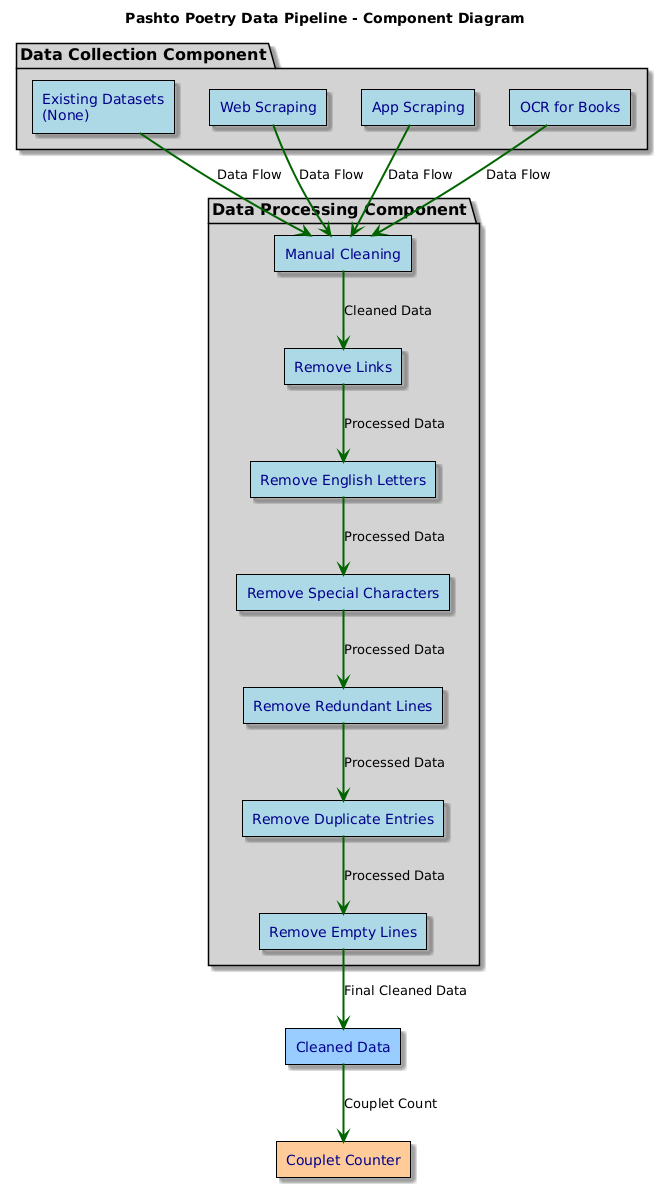
\includegraphics[width=0.35\textwidth]{datapipeline.png}
    \caption{Data Cleaning Pipeline}
    \label{fig:data-pipeline}
\end{figure}

All the data was then cleaned and sorted to get just the Pashto poetry of each poet. All in all, we were able to collect 27,607 couplets from a total of 23 poets. The chosen poets also show a good distribution in the sense that some poets are of historic ages such as Rahman Baba, Khushal Khan Khattak, and Hamza Baba, while there are also recent poets such as Ghani Khan, and Khatir Afridi. Thus, the poetry would have varying styles, themes, word usage, dialects, and vocabulary which would help in training a robust model as the patterns would be more diverse. 

The table below shows the number of couplets collected for each poet.
\begin{table}[H]
    \centering
    \begin{tabular}{|c|p{10em}|c|}
        \hline
        \rowcolor{lightgray} \textbf{No.} & \textbf{Poet/Shayari} & \textbf{Couplets Count} \\ \hline
        1. & Abbasin Yousuf & 1875 \\ \hline
        2. & Ajmal Khattak & 780 \\ \hline
        3. & Allama Abdul Hai & 2380 \\ \hline
        4. & Aziz Mazerwal & 30 \\ \hline
        5. & Ghani Khan & 1399 \\ \hline
        6. & Hamza Baba & 1177 \\ \hline
        7. & Javed Ahmedzai & 561 \\ \hline
        8. & Karan Khan & 979 \\ \hline
        9. & Khaliq Ziari & 40 \\ \hline
        10. & Khatir Afridi & 1436 \\ \hline
        11. & Khushal Khan Khattak & 4257 \\ \hline
        12. & Matiullah Turab & 1192 \\ \hline
        13. & Mumtaz Orakazi & 1645 \\ \hline
        14. & Munir Jan & 1169 \\ \hline
        15. & Naeem Ahmed & 856 \\ \hline
        16. & Rabia Mumtaz & 572 \\ \hline
        17. & Rahman Baba & 2202 \\ \hline
        18. & Rehmat Shah & 1534 \\ \hline
        19. & Sahib Shah Sabir & 1051 \\ \hline
        20. & Shabbir Khan Durrani & 1056 \\ \hline
        21. & Shakir Orakzai & 569 \\ \hline
        22. & Salim Riaz & 232 \\ \hline
        23. & Shoaib Khan Khattak & 615 \\ \hline
        \cellcolor{lightgray} \textbf{Total} & & \textbf{27,607} \\ \hline
    \end{tabular}
    \caption{Poets and their couplets count}
    \label{tab:poets-couplets-table}
\end{table}

The histogram below shows the distribution of the poets in the dataset.
\begin{figure}[H]
    \centering
    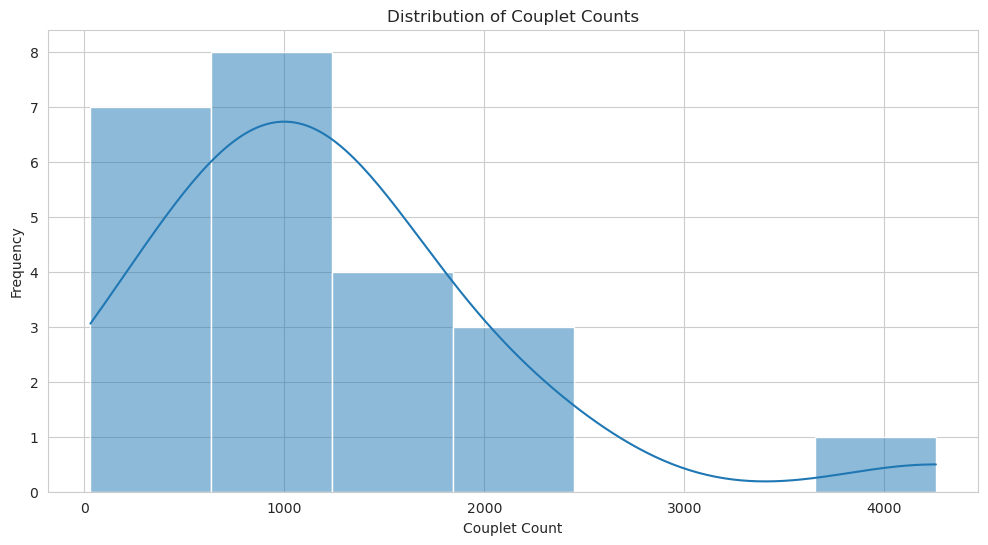
\includegraphics[width=0.475\textwidth]{poet_dist_hist.png}
    \caption{Poet Distribution}
    \label{fig:poet-dist-hist}
\end{figure}
It shows that the dataset is imbalanced, with some poets having a very high number of couplets, while some poets have a very low number of couplets. This imbalance in the dataset could lead to the models overfitting on the poets with a high number of couplets, and not learning the features of the poets with a low number of couplets well enough.

We also decided to remove 3 of the poets for our models with the lowest poet count - mainly Aziz Mazerwal, Khaliq Ziari, and Salim Riaz. The final dataset that we trained our models on consisted of 20 poets then. 

\subsection{Machine Learning Models}
From our extensive literature review, we found that machine learning models have been widely used for classification and attribution tasks. Thus, we decided to employ several machine learning models to classify Pashto poetry. Our main machine learning pipeline includes first label encoding the dataset, followed by extracting features from the text data based on TF-IDF Feature Extraction. TF-IDF Feature Extraction works by first tokenizing the text data, followed by converting the text data into a matrix of token counts, and then normalizing the token counts. The TF-IDF value increases proportionally to the number of times a word appears in the document but is offset by the frequency of the word in the corpus. This helps in reducing the importance of common words in the text data. For our models, we extracted 10000 features. The TF-IDF vectors were then split into 80-20 train-test split. Since our dataset was heavily imbalanced, we decided to go for a weighted train-test split, where the train-test split was done in such a way that the distribution of the classes in the train and test set was the same, thus, each class had the same ratio of samples in the train and test set. Finally, those TF-IDF vectors were then passed through several machine learning models including Random Forest, Support Vector Machine, Logistic Regression, and XGBoost, as they all were supported by the literature. The diagram below explains the complete machine learning pipeline.

\begin{figure}[H]
    \centering
    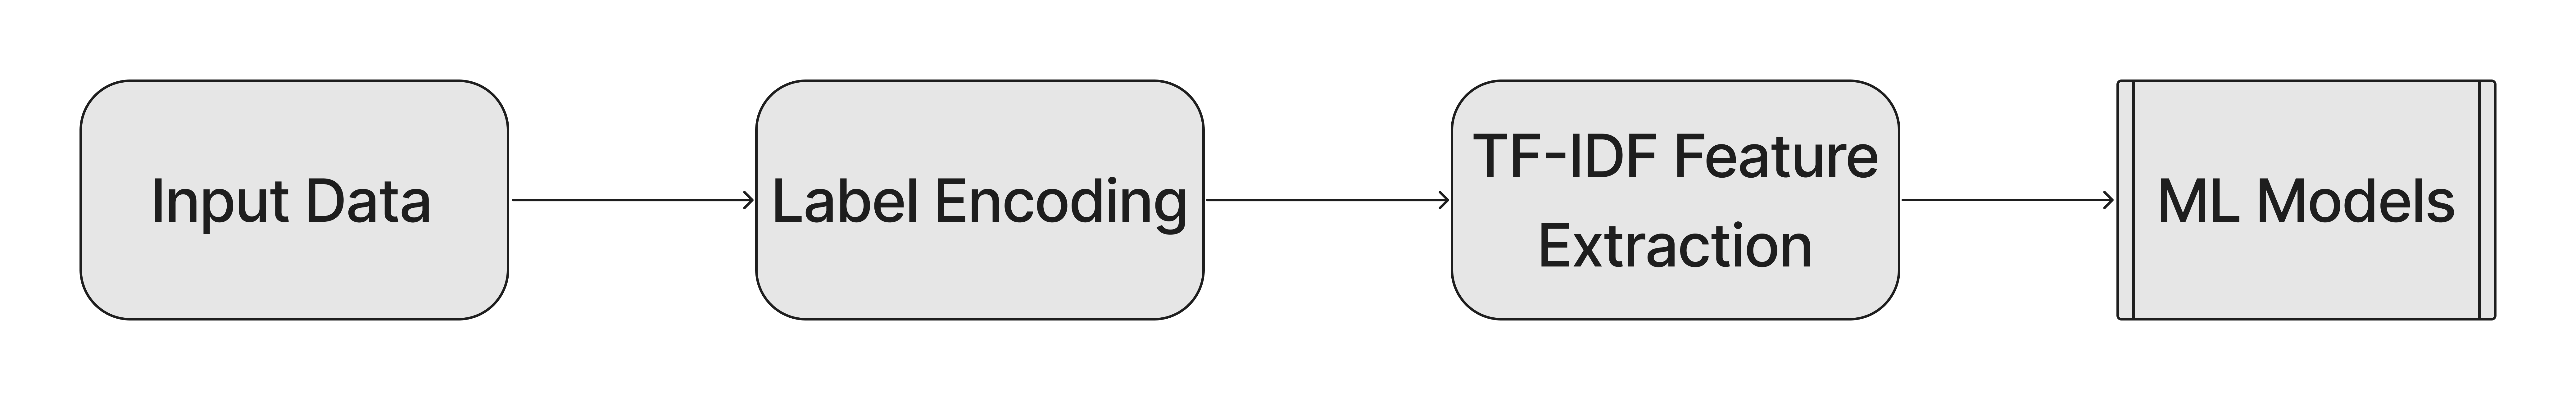
\includegraphics[width=0.45\textwidth]{ml_pipe.png}
    \caption{Machine Learning Pipeline}
\end{figure}

We used python's ``Pandas'' library for creating the dataframes, and for labelling the data for the 20 poets. We defined our own weighted train-test split function to ensure that the distribution of the classes in the train and test set was the same. Python's ``TfidfVectorizer'' was used for the TF-IDF feature extraction. Lastly, we used the ``Scikit-learn'' library for the machine learning models, and the ``XGBoost'' library for the XGBoost model.

\subsubsection{Random Forest}
Random Forest is an ensemble learning method that operates by constructing a multitude of decision trees at training time and outputting the class that is the mode of the classes of the individual trees. Random Forest is a bagging technique and is an ensemble of decision trees. We trained our Random Forest model on 100 esimators, with no max-depth defined. We tried hyperparameter tuning of the Random Forest model as well with various parameters, however, they did not improve the model performance. 

\subsubsection{Support Vector Machine}
Support Vector Machine is a supervised machine learning algorithm that can be used for both classification or regression challenges. From the literature, we found that SVM has been widely used for text classification tasks. We experimented with the linear kernel, rbr kernel with gamma set to scale and C set to 1 as this was the best performing hyperparameters for our dataset.

\subsubsection{Logistic Regression}
Logistic Regression is a statistical model that in its basic form uses a logistic function to model a binary dependent variable. We used the Logistic Regression model on 1000 iterations, we also implemented a liblinear solver, and a newton-cg solver with a C value of 10. 

\subsubsection{XGBoost}
XGBoost is an optimized distributed gradient boosting library designed to be highly efficient, flexible, and portable. It implements machine learning algorithms under the Gradient Boosting framework. We used the XGBoost model with 100 n estimators, a max depth of 3, a learning rate of 0.1, gamma set to 0.1, eval metric set to logloss, and a scale pos weight of 1, as this was the best performing hyperparameters for our dataset.


\subsection{Deep Learning Models}
We also experimented with deep learning models for Pashto poetry classification. Deep Learning models are inspired by the structure and function of the brain, in which the neural networks work in a similar way to the human brain, updating and learning their weights and biases based on the input data. As such, deep learning models have been quite powerful, and robust in their ability to learn complex patterns in the data. Therefore, they have also been widely used for text classification tasks.  

We used the Keras library with TensorFlow backend for our deep learning models. Our deep learning pipeline included first labelling and one-hot encoding the input data, followed by tokenizing the text data, and then padding the text data to a fixed length. We then used an embedding layer to convert the text data into a dense vector of fixed size. Those embeddings were then passed through our deep learning models. The figure below illustrates the complete deep learning pipeline.

\begin{figure}[H]
    \centering
    
\includegraphics[width=0.45\textwidth]{dl_pipe.png}
    \caption{Deep Learning Pipeline}
\end{figure}

We used the ``Pandas'' library for creating the dataframes. The ``Label Encoder'' was used for label encoding the 20 poets in our dataframes. We used our previous weighted train-test split function for splitting the data into train, validation and test sets. We used an 75-5-20 train-validation-test split. The remaining methodology remains the same for tokenization, padding, and embedding layers. We used the ``Keras'' library for the deep learning models, and the ``TensorFlow'' library for the backend.

We initially thought of using Bi-LSTM, Bi-GRU, and CNN models for our deep learning pipeline. However, after various experimentation and hyperparameter tuning, we found that those deep learning models were not performing well on our dataset, mostly overfitting on the training data due to which we were not getting a desired validation or test accuracy as expected. Therefore, after experimenting with the Bi-LSTM model, we decided to move onto other Deep Learning models instead. 

\subsubsection{Bi-LSTM}
For the Bi-LSTM model, we used 3 Bi-LSTM layers with 64, 32, and 16 units respectively. We also used a dropout layer with a dropout rate of 0.3 after each Bi-LSTM layer. We used the softmax activation function for the output layer. We used the Adam optimizer with a learning rate of 0.001, and sparse categorical cross-entropy as the loss function. We used early stopping with a patience of 10 epochs. We trained the model for 20 epochs with a batch size of 32. We also experimented with various hyperparameters for the Bi-LSTM model, including the number of units, the number of layers, the dropout rate, the learning rate, and the batch size. We also implemented a simple LSTM model, however, the Bi-LSTM model performed better than the simple LSTM model, but even that was overfitting on the training data. We suspect the overfitting was due to the small dataset size, and similar features in the poetry of different poets. Therefore, we decided not to move on with more traditional deep learning models and instead move on to transformer models instead.


\subsection{Transformer Models}

Tranformers are a type of deep learning model aimed at solving natural language processing, and other sequence-based tasks such as text classification, generation, and translation. Transformers have been widely used for text classification tasks due to their ability to learn long-range dependencies in the data. They utilize the power of attention, and encoder decoder architecture. As from our literature review, transformer based models can be seen to perform well in the recent papers for text classification tasks, we decided to experiment with transformer models for Pashto poetry classification. We experimented with a few transformer based models; DistilBERT, Bert based Multilingual Uncased, Meta Llama3.2-1B, Mt5 Multilingual XLSum, and Mt0 Base.

The methodology remains the same as for the Deep Learning models, since transformers are essentially deep learning models. We used the ``Pandas'' library for creating the dataframes. The ``Label Encoder'' was used for label encoding the 20 poets in our dataframes. We used our previous weighted train-test split function for splitting the data into train, validation and test sets. We used an 80-10-10 train-validation-test split. The remaining methodology remains the same for tokenization, padding, and embedding layers where needed. We used the ``Hugging Face'' library for the transformer models, and the ``TensorFlow'' library for the backend. 


% \subsubsection{roBERTa}
% roBERTa is a robustly optimized BERT approach, which is a transformer-based model. It is a variant of BERT, and has been pre-trained on a large corpus of text data. We used the ``Hugging Face'' library for the roBERTa model.


\subsubsection{DistilBERT}
DistilBERT is a distilled version of BERT, which is a transformer-based model. It is a smaller version of BERT, and has been pre-trained on a large corpus of text data. We used the ``Hugging Face'' library for the DistilBERT model. 


\subsubsection{Meta Llama}
We used the Meta Llama 3.2 model, which is collection of multilingual large language models (LLMs) is a collection of pretrained and instruction-tuned generative models in 1B (billion parameters) and 3B (billion parameters) sizes (text in/text out). The Llama 3.2 instruction-tuned text only models are optimized for multilingual dialogue use cases, including agentic retrieval and summarization tasks. They outperform many of the available open source and closed chat models on common industry benchmarks. For our task, we opted for the 1B model. We used the ``Hugging Face'' library for the Meta Llama model. 

\subsubsection{Bert Based Multilingual Uncased}
We also tried the Bert Based Multilingual Uncased model, a pretrained model of 168M (million) parameters, on the top 102 languages with the largest Wikipedia using a masked language modeling (MLM) objective. The MLM model takes a sentence, and randomly masks 15\% of the words in the input then run the entire masked sentence through the model and has to predict the masked words. This is different from traditional recurrent neural networks (RNNs) that usually see the words one after the other, or from autoregressive models like GPT which internally mask the future tokens. It allows the model to learn a bidirectional representation of the sentence. We used the ``Hugging Face'' library for the Bert Based Multilingual Uncased model.

\subsubsection{Mt5 Multilingual XLSum} 
The Mt5 Multilingual XLSum is based on Google's Mt5 model, which is a checkpoint finetuned on the 45 languages of the \href{https://huggingface.co/datasets/csebuetnlp/xlsum}{XLSum Dataset}, which includes Pashto as well. 

\subsubsection{Mt0 Base}
We also trained the Mt0 Base model by bigscience, based on BLOOMZ and mT0, a family of models capable of following human instructions in dozens of languages zero-shot. They fintuned BLOOM and mt5 pretrained multilingual models on their crosslingual task mixture (xP3), and found that their resulting model was capable of crosslingual generalization to unseen tasks and languages. Their model is finetuned on 101 languages, including Pashto, hence we decided to experiment with this model as well.

\section{Results}

In this section we explore and discuss the results of our experiments with the machine learning, deep learning, and transformer models for Pashto poetry classification. We present the results of our experiments in the following subsections. 

\subsection{Machine Learning Models}

This subsection presents the results of our experiments with the machine learning models. We used the following machine learning models for our experiments: Random Forest, Support Vector Machine, Logistic Regression, and XGBoost. The dataset was divided into 21844 samples for training, and 5465 samples for testing. The models were trained on an 8 Core, 4.90 GHz Intel Core i7-12700 CPU with 16GB RAM. 

\subsubsection{Random Forest}
Using 100 estimators, and a max depth of None, the Random Forest model achieved an accuracy of 51.93\%, and an F1 score of 0.50. The confusion matrix for the Random Forest model is shown below:
\begin{figure}[H]
    \centering
    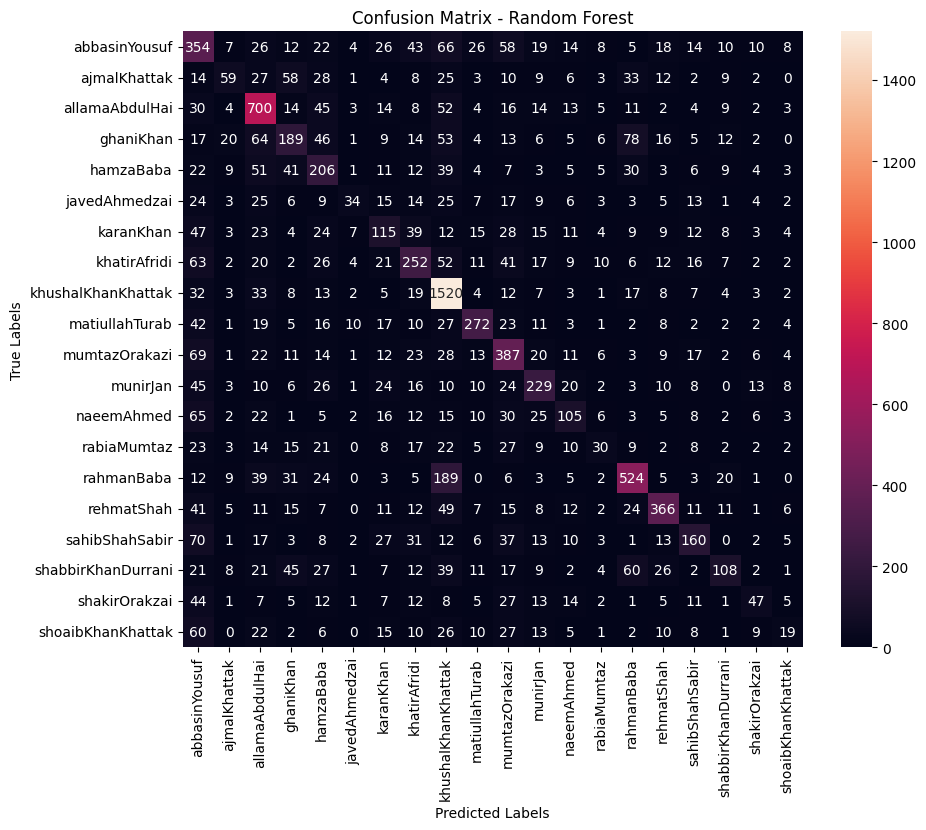
\includegraphics[width=0.45\textwidth]{rf_confmat.png}
\end{figure}

\subsubsection{Support Vector Machine}
With a C value of 1.0, an `rbf' kernel, and a gamma value of `scale', the Support Vector Machine model achieved an accuracy of 61.92\%, and an F1 score of 0.60. The confusion matrix for the Support Vector Machine model is shown below:
\begin{figure}[H]
    \centering
    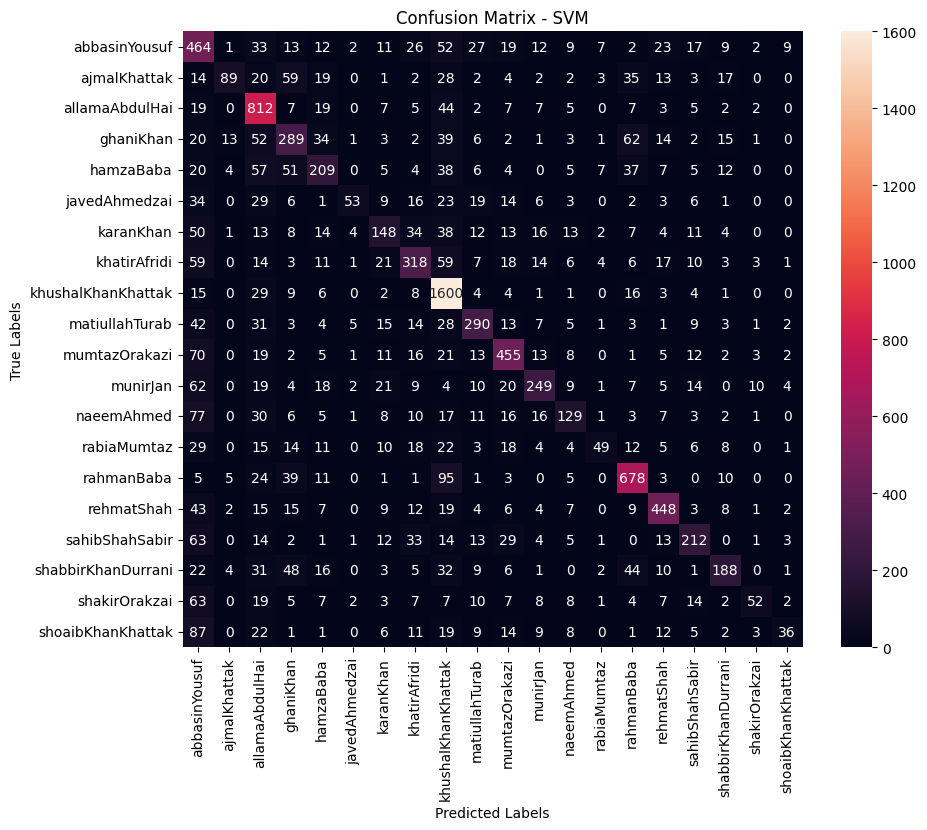
\includegraphics[width=0.45\textwidth]{svm_confmat.png}
\end{figure}

\subsubsection{Logistic Regression}
For the Logistic Regression model, our best hyperparameters turned out to be a C value of 10, max iterations of 1000, and a `newton-cg' solver. This gave an accuracy of 62.88\%, and an F1 score of 0.62. The confusion matrix for the Logistic Regression model is shown below:
\begin{figure}[H]
    \centering
    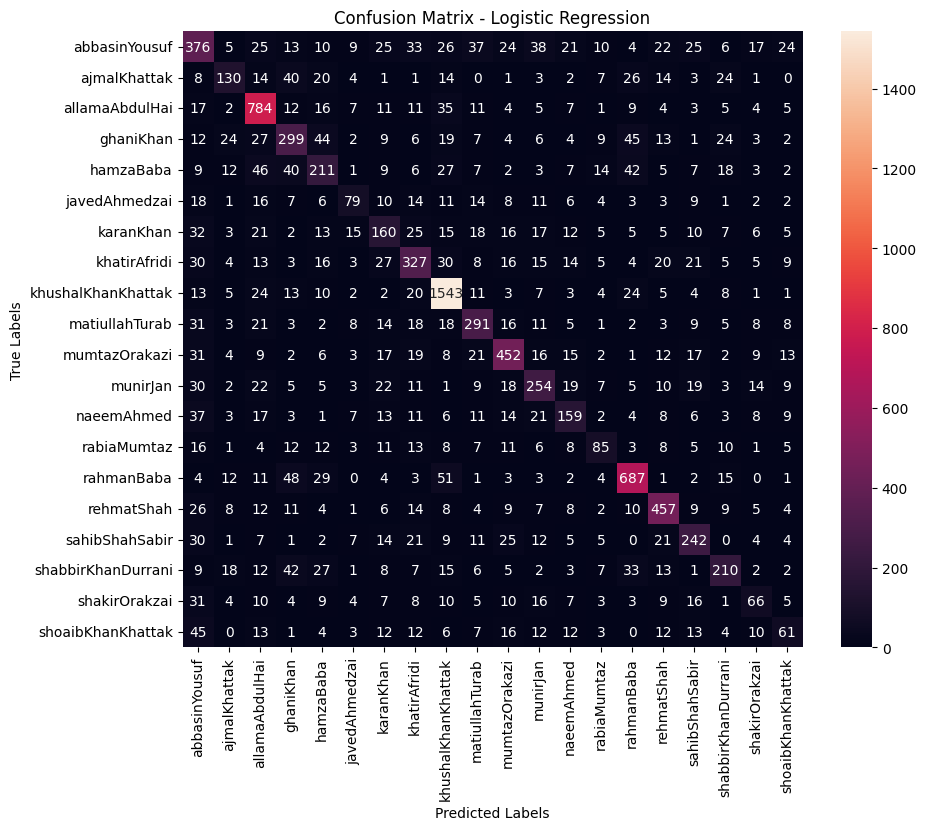
\includegraphics[width=0.45\textwidth]{logreg_confmat.png}
\end{figure}

\subsubsection{XGBoost}
Our best hyperparameters for XGBoost were 100 estimators, a learning rate of 0.1, max depth of 3, gamma value of 0.1, and a log-loss evaluation metric. This gave us an accuracy of 41.67\% and an F1 Score of 0.38. The confusion matrix for the XGBoost model is shown below:
\begin{figure}[H]
    \centering
    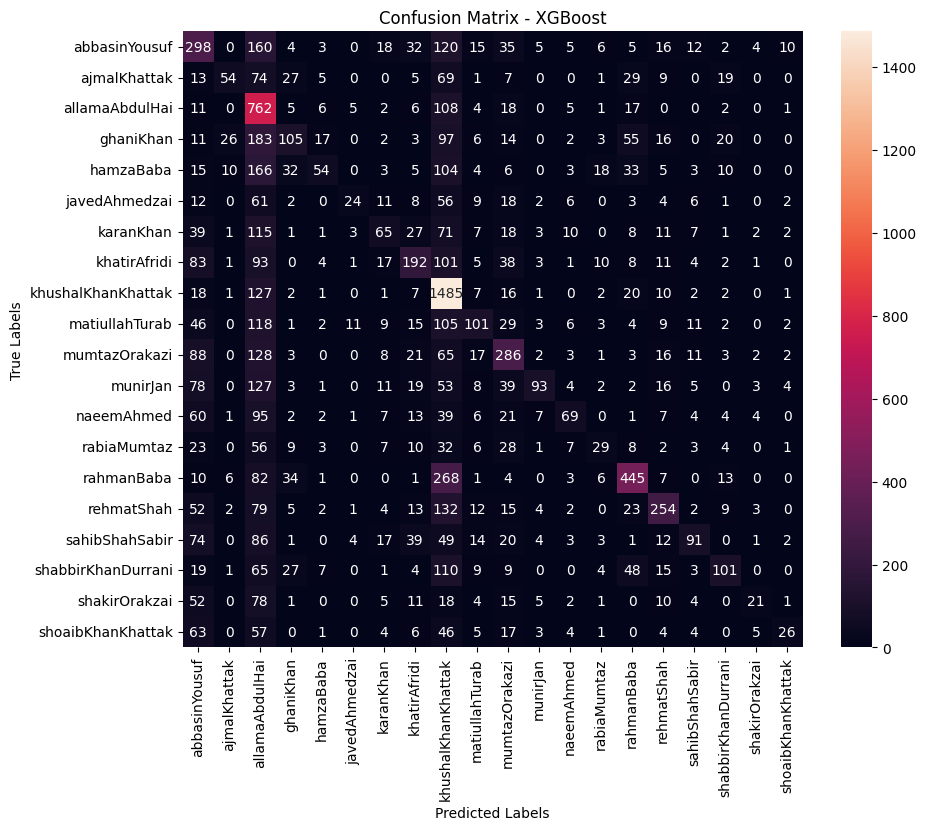
\includegraphics[width=0.45\textwidth]{xgboost_confmat.png}
\end{figure}

\subsection{Deep Learning Models}

This subsection presents the results of our experiments with the deep learning models. We used the following deep learning models for our experiments: LSTM and Bi-LSTM. The dataset was divided into 19111 samples for training, 2727 samples for validation, and 5471 samples for testing. They were trained on 2 Tesla T4 GPUs available on Kaggle, with Kaggle's 29GB RAM. 

\subsubsection{LSTM}
We experimented with various layers, and hyperparameters for LSTM including Bi-LSTM layers as well. The models were trained on 20 Epochs, with early stopping enabled. We experimented with a simple LSTM model with 2 LSTM layers of 128 and 64 units, respectively. We also added 2 dropout layers, and a dense layer with 64 units. The model was overfitting the training data, hence we continued with different parameters including compiling with an Adam Optimizer with a learning rate of 0.001, and a sparse categorical cross entropy loss, but that as well overfitted with a poor accuracy on the validation and test sets. Our final model was a Bi-LSTM model with a Dense layer with a softmax activation function, compiled using the Adam Optimizer with a learning rate of 0.0001, sparse categorical cross entropy loss, and an early stopping layer. The model achieved an accuracy of 59.63\% on the test set. The plots and confusion matrix for the Bi-LSTM Model are shown as follows:

\begin{figure}[H]
    \centering
    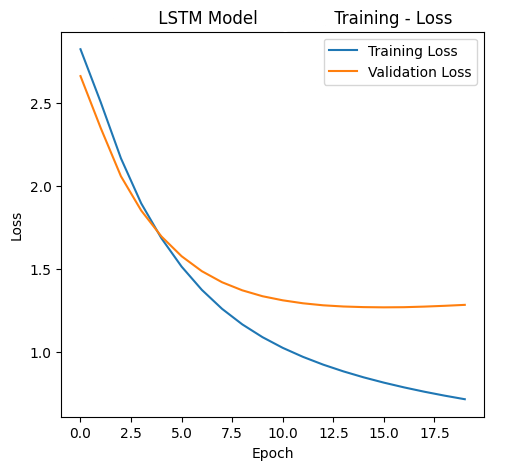
\includegraphics[width=0.4\textwidth]{dl_lstm_trainloss.png}
    \caption{Training Loss for LSTM Model}
    \label{fig:dl_lstm_trainloss}
\end{figure}

\begin{figure}[H]
    \centering
    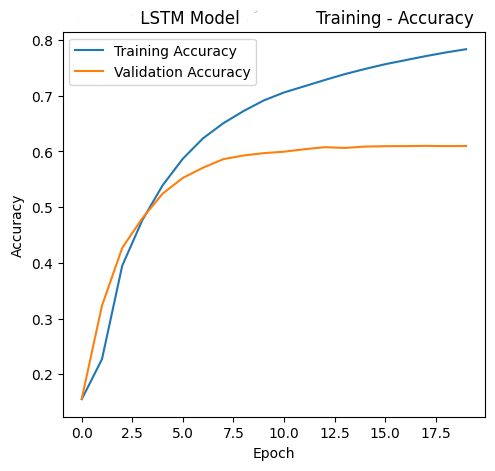
\includegraphics[width=0.4\textwidth]{dl_lstm_trainaccuracy.png}
    \caption{Training Accuracy for LSTM Model}
    \label{fig:dl_lstm_trainaccuracy}
\end{figure}

\begin{figure}[H]
    \centering
    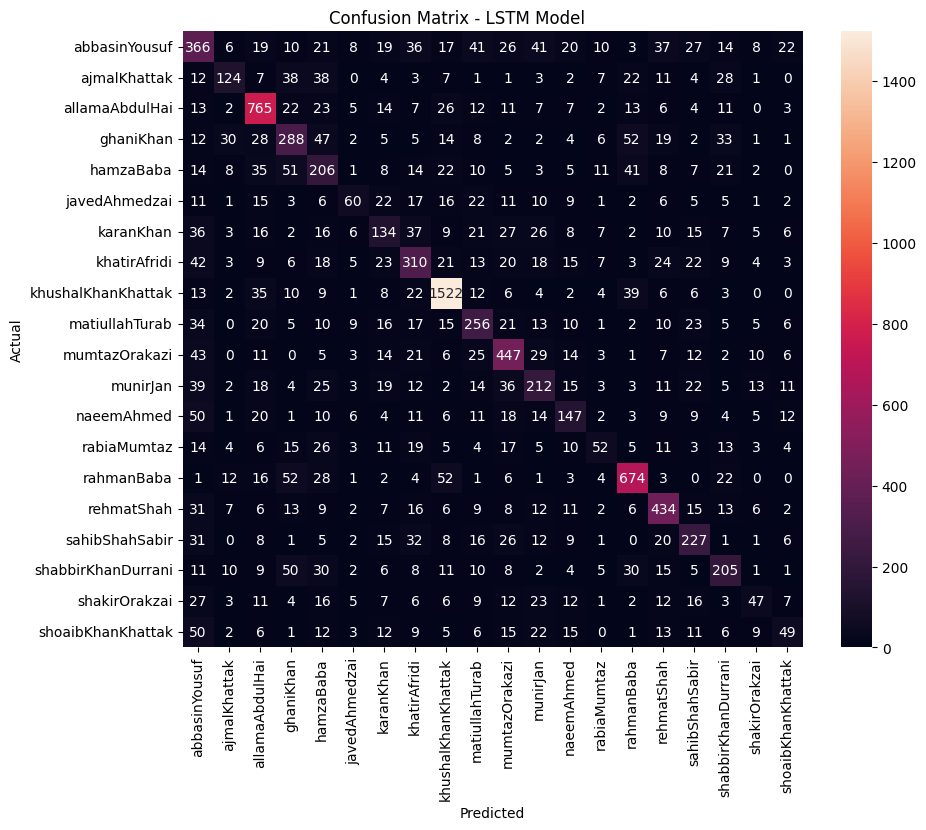
\includegraphics[width=0.45\textwidth]{dl_lstm_confmat.png}
    \caption{Confusion Matrix for LSTM Model}
    \label{fig:dl_lstm_confmat}
\end{figure}

\subsection{Transformer Models}

This subsection presents the results of our experiments with the transformer models. We used the following transformer models for our experiments: roBERTa, DistilBERT, and Meta Llama-3.2-1b. The embeddings generated were trained on 2 Tesla T4 GPUs available on Kaggle, with Kaggle's 29GB RAM.

\subsubsection{roBERTa}

\subsubsection{DistilBERT}

\subsubsection{Meta Llama-3.2-1b}

The Meta Llama 3.2 1b parameter model was trained on 20 epochs, with a batch size of 8, learning rate of 0.001, the Adam optimizer, and cross entropy loss function, with an early stopping. The model only achieved an accuracy of 48.88\%. The plots and confusion matrix for the Meta Llama-3.2-1b Model are shown as follows:

\begin{figure}[H]
    \centering
    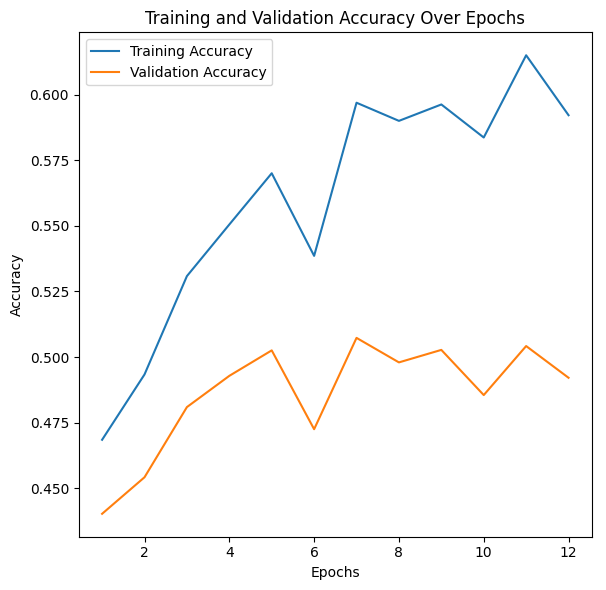
\includegraphics[width=0.4\textwidth]{llama_trainloss.png}
    \caption{Training Loss for Meta Llama-3.2-1b Model}
    \label{fig:llama_trainloss}
\end{figure}

\begin{figure}[H]
    \centering
    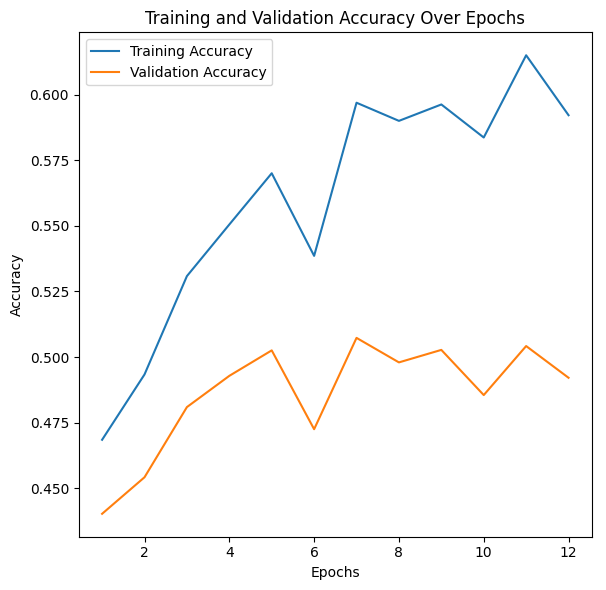
\includegraphics[width=0.4\textwidth]{llama_trainaccuracy.png}
    \caption{Training Accuracy for Meta Llama-3.2-1b Model}
    \label{fig:llama_trainaccuracy}
\end{figure}

\begin{figure}[H]
    \centering
    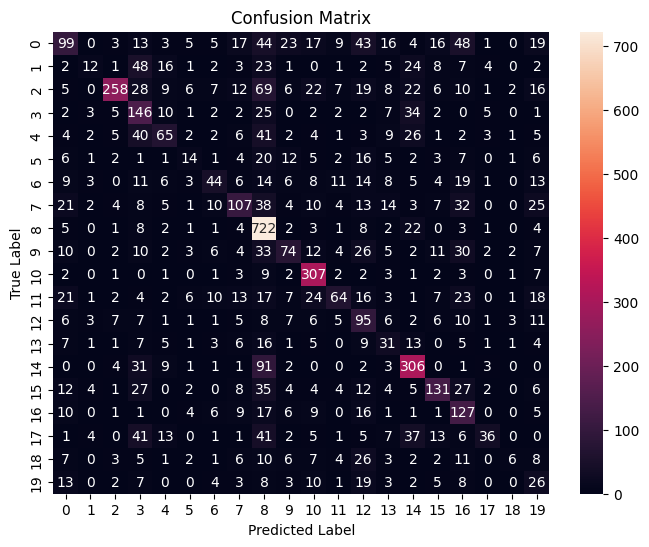
\includegraphics[width=0.45\textwidth]{llama_confmat.png}
    \caption{Confusion Matrix for Meta Llama-3.2-1b Model}
    \label{fig:llama_confmat}
\end{figure}

\subsection{Bert Based Multilingual Uncased}
As above, the model was trained on 20 epochs, with a batch size of 8, learning rate of 0.001, the Adam optimizer, and cross entropy loss function, with an early stopping. The model only achieved an accuracy of 45.61\%. The plots and confusion matrix for the Bert Based Multilingual Uncased Model are shown as follows:

\begin{figure}[H]
    \centering
    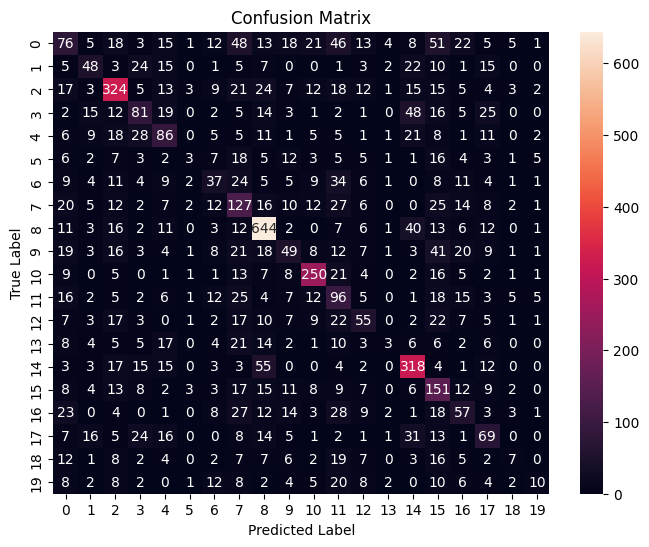
\includegraphics[width=0.45\textwidth]{bbmu_confmat.png}
    \caption{Confusion Matrix for Bert Based Multilingual Uncased Model}
    \label{fig:bbmu_confmat}
\end{figure}

\begin{figure}[H]
    \centering
    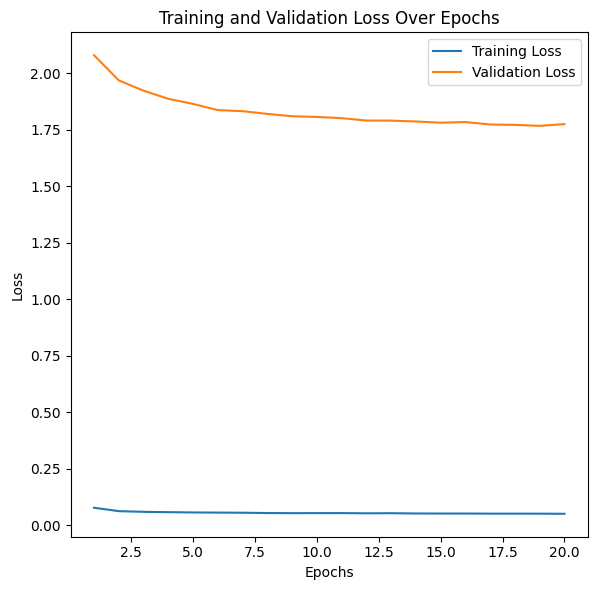
\includegraphics[width=0.4\textwidth]{bbmu_trainloss.png}
    \caption{Training Loss for Bert Based Multilingual Uncased Model}
    \label{fig:bbmu_trainloss}
\end{figure}

\begin{figure}[H]
    \centering
    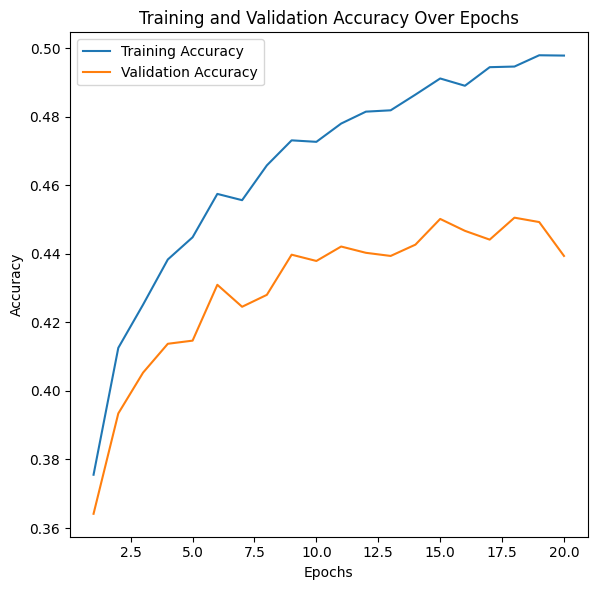
\includegraphics[width=0.4\textwidth]{bbmu_trainaccuracy.png}
    \caption{Training Accuracy for Bert Based Multilingual Uncased Model}
    \label{fig:bbmu_trainaccuracy}
\end{figure}

\subsection{Summary of Results}

This subsection presents a summary of the results of our experiments with the machine learning, deep learning, and transformer models for Pashto poetry classification.

\begin{table}[ht]
    \centering
    \begin{tabular}{|l|c|}
        \hline
        \textbf{Model} & \textbf{Accuracy} \\
        \hline
        Logistic Regression & 62.88\% \\
        Support Vector Machine & 61.92\% \\
        Bi-LSTM & 59.63\% \\
        Random Forest & 51.93\% \\
        Meta Llama-3.2-1b & 48.88\% \\
        Bert Based Multilingual Uncased & 45.61\% \\
        XGBoost & 41.67\% \\
        \hline
    \end{tabular}
    \caption{Table of Results}
    \label{tab:results}
\end{table}






\section{Discussion and Analysis}
In this section we discuss the results of the experiments and analyze the performance of the models. We also discuss the limitations of the models and the dataset used in the experiments.

We had initially expected the Deep Learning and Transformer Models to perform better on the data. Unexpectedly, however, two of the machine learning models; Logistic Regression and Support Vector Machine, outperformed the Deep Learning and Transformer models. The Logistic Regression model had the highest accuracy of 62.88\% and the Support Vector Machine model had the second highest accuracy of 61.92\%. The Bi-LSTM model trained on the TF-IDF features that were used for the machine learning model performed the third best with an accuracy of 59.63\%. We suspect this might be due to the inherent similar features of the various classes within the data. As such, the TF-IDF feature extractor might be better at capturing these features than the Transformer and Deep Learning models. Also an notable observation we made from our confusion matrices is that all the models tend to follow a similar pattern in terms of accuracy for the different classes. The older poets, mainly, Allama Abdul Hai, Ghani Khan, Kushal Khan Khattak, Mumtaz Orakazi, Rahman Baba, and Rehmat Shah had the highest accuracy across all models. That is, all of the models predicted these poets with the highest accuracy, and all the models predicted the newer poets very poorly. This also strengthens our belief in the inherent similarity between the data as the older poets might use a different style of poetry, while the newer poets might use a modern and similar style of poetry which might be harder to differentiate. Another reason for the poor performance could be the scarcity of data. All models predict Kushal Khan Khattak with the highest accuracy, which might be due to the fact that he has the most number of couplets in the dataset - 4257. All other poets have couplet counts less than 2000, apart from 2 poets with a couplet count of 2380 and 2202. This vast distribution of data might have caused the models to overfit on the data of Kushal Khan Khattak, and not learn the features of the other poets well enough. The data distribution can be referred to from \hyperref[fig:poet-dist-hist]{Section III.A}. 

\section{Future Work}

% \input{conclusion}

\bibliographystyle{ieeetr}
\bibliography{ref}

\end{document}

